%---------------------------------------------------------------------------
%	UNIVERSIDADE FEDERAL DE UBERLÂNDIA
%	Faculdade de Engenharia Elétrica
%	Programa de Pós-Graduação em Engenharia Elétrica
%	Laboratório de Engenharia Biomédica
%	Dissertação de Mestrado
%	Capítulo 4: Resultados
%---------------------------------------------------------------------------
\section{Resultados}
Após a construção do problema no FEMM, foi executado o gerador de malhas
\begin{figure}[H]
\centering
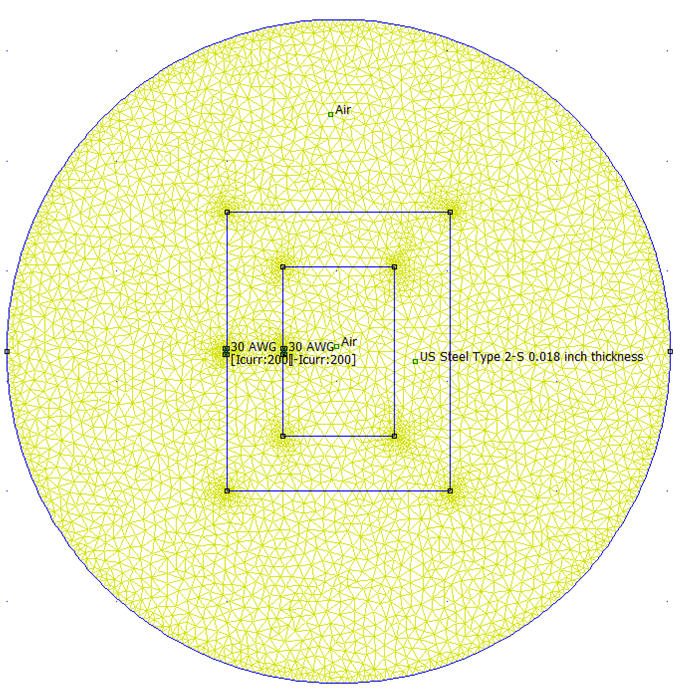
\includegraphics[scale=0.5]{img/assig1/femm_2.png}
\caption[Malha de pontos gerada pelo FEMM]{Malha de pontos gerada pelo FEMM.}
\label{femm2}
\end{figure}

\begin{figure}[H]
\centering
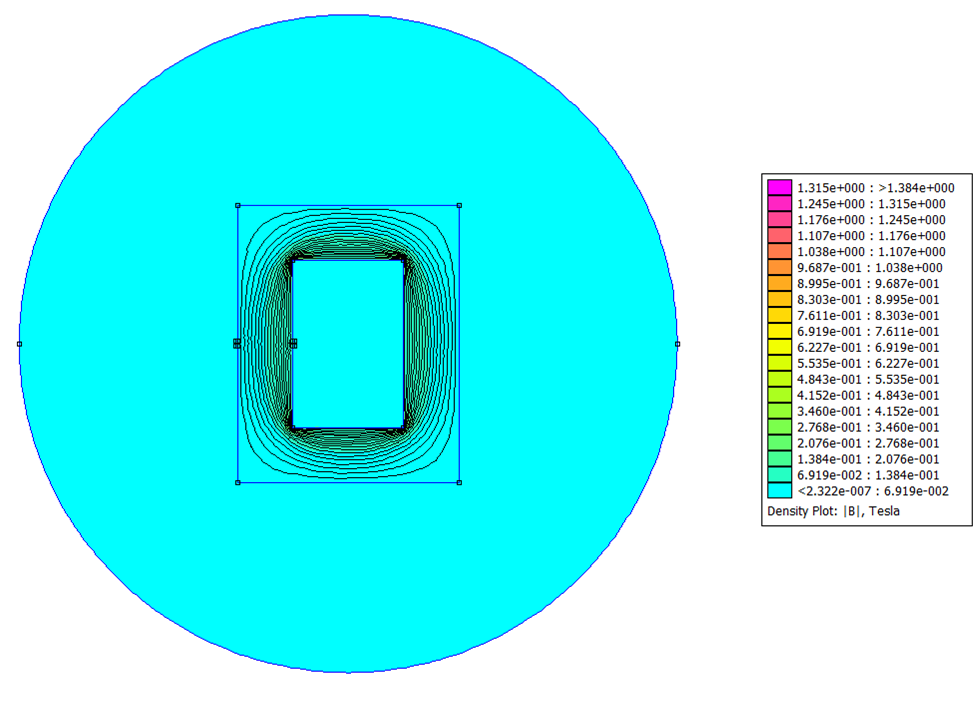
\includegraphics[scale=0.5]{img/assig1/femm_4.png}
\caption[Densidade de fluxo (Mapa de calor)]{Densidade de fluxo (Mapa de calor).}
\label{femm3}
\end{figure}

\subsection{Análise do fluxo magnético, potencial e da intensidade de campo a partir de uma linha reta que passa pelo eixo central do circuito magnético}

Para realizar a análise do fluxo magnético, potencial e da intensidade de campo, foi inserida no circuito magnético uma linha reta que coincide com o eixo central do mesmo, conforme ilustrado na figura \ref{loc_med}. Os gráficos das figuras \ref{graf_dfm}, \ref{graf_pot} e \ref{graf_ic} apresentam, respectivamente, a densidade de fluxo magnético (B), o potencial e a intensidade de corrente (H).

\begin{figure}[H]
\centering
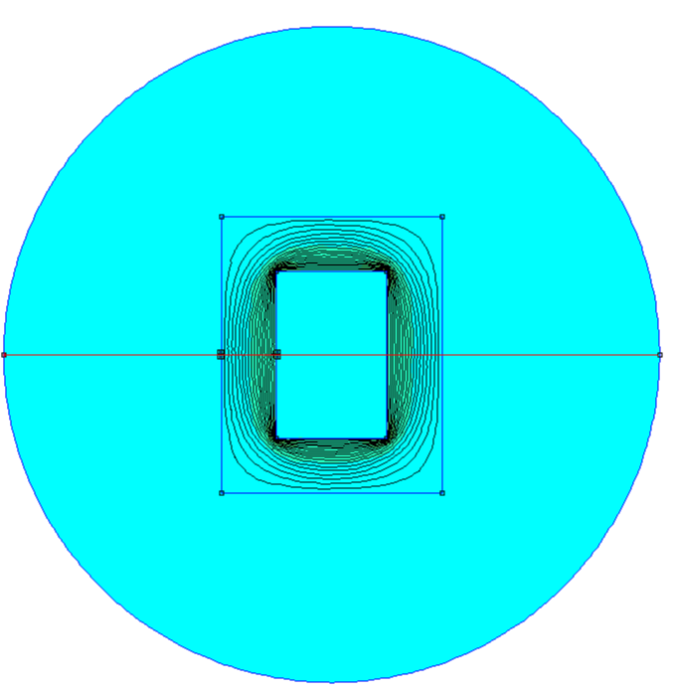
\includegraphics[scale=0.65]{img/assig1/linha_1.png}
\caption[Local de medição]{Local de medição.}
\label{loc_med}
\end{figure}

\begin{figure}[H]
\centering
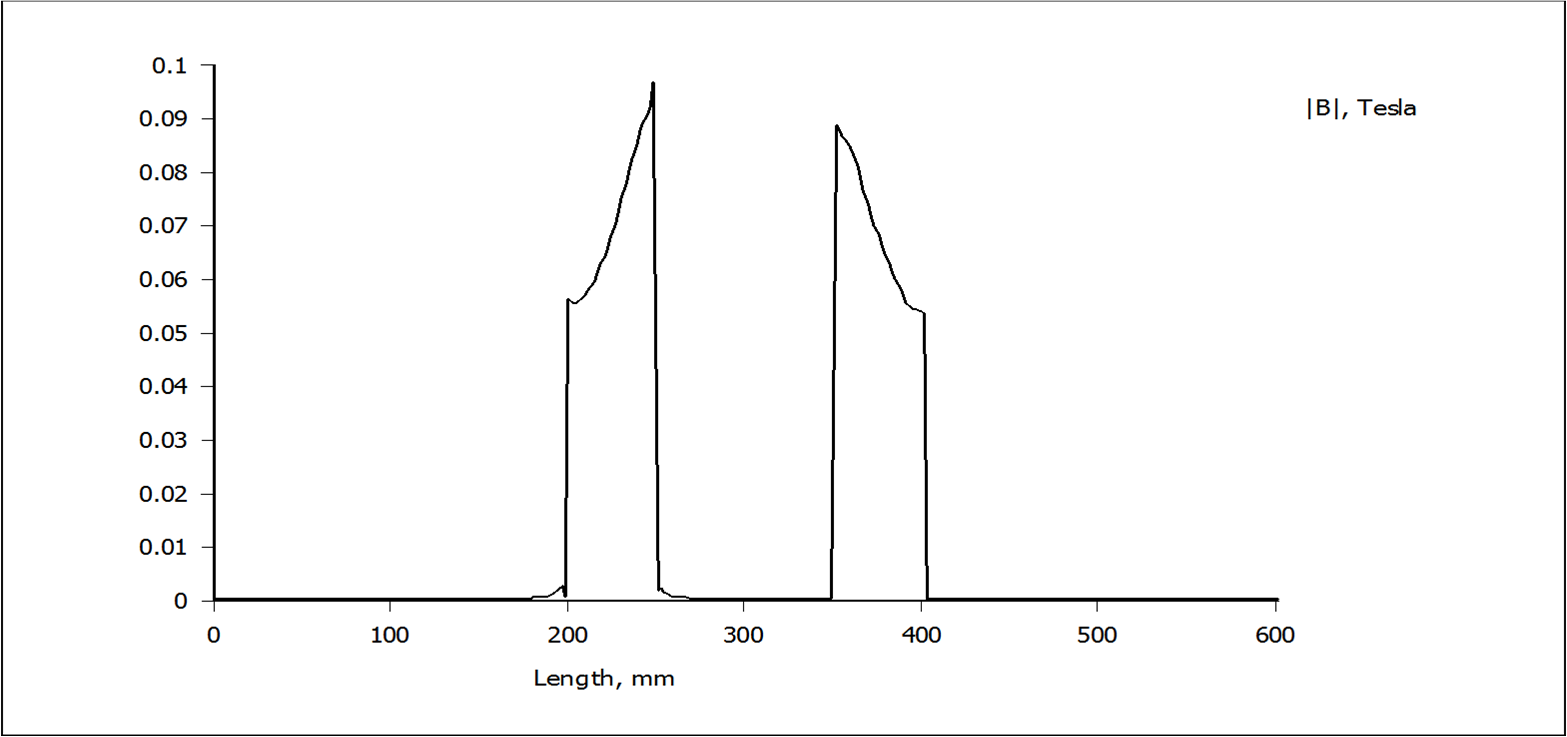
\includegraphics[scale=0.3]{img/assig1/linha_B.png}
\caption[Gráfico da densidade de fluxo magnético]{Gráfico da densidade de fluxo magnético.}
\label{graf_dfm}
\end{figure}

\begin{figure}[H]
\centering
\includegraphics[scale=0.3]{img/assig1/linha_pot.png}
\caption[Gráfico do potencial]{Gráfico do potencial.}
\label{graf_pot}
\end{figure}

\begin{figure}[H]
\centering
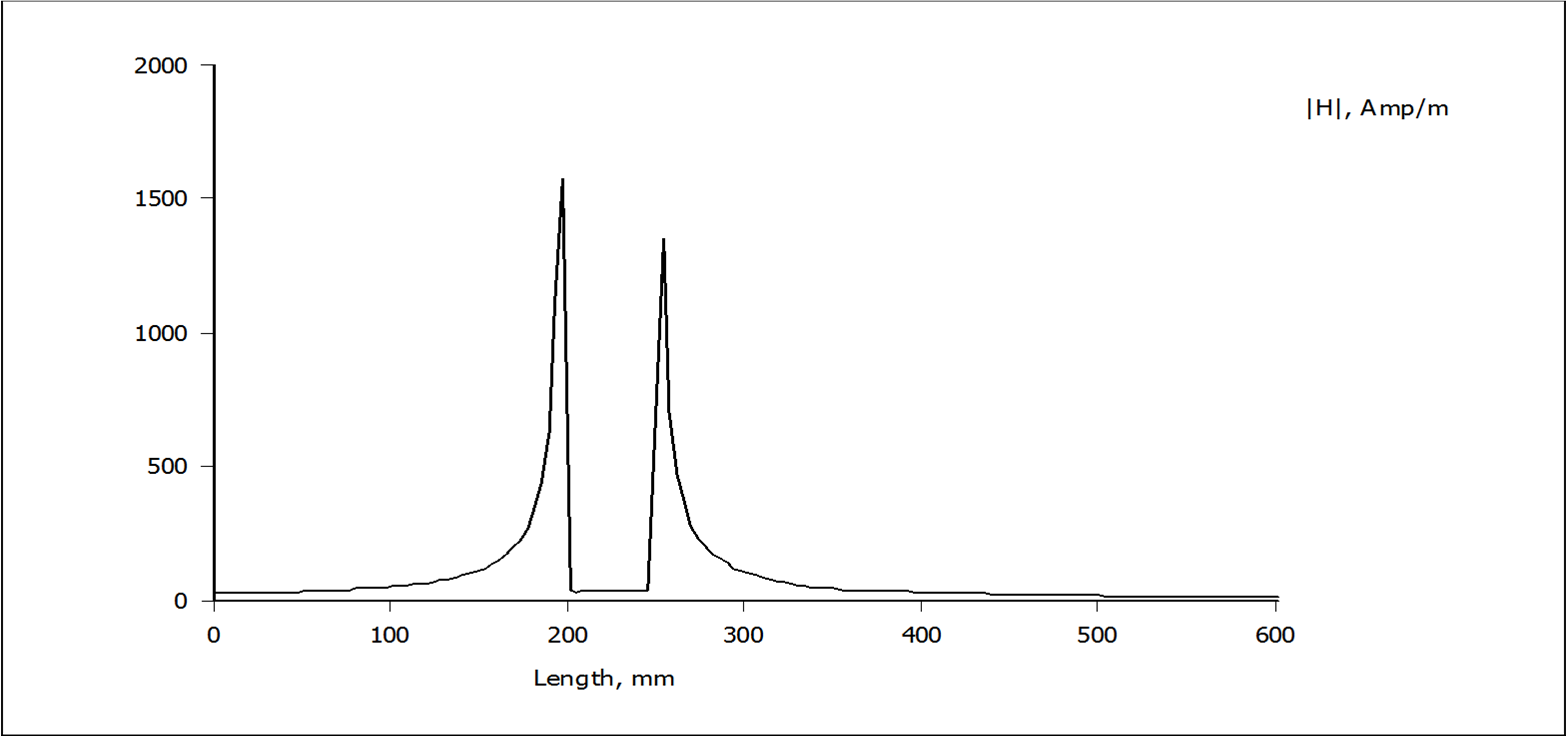
\includegraphics[scale=0.3]{img/assig1/linha_H.png}
\caption[Gráfico da intensidade de campo]{Gráfico da intensidade de campo.}
\label{graf_ic}
\end{figure}

\subsubsection{Análise para a corrente do circuito com módulo igual a 0.2 [A]}
Para comparar a influência da corrente na análise, foi realizada uma segunda análise utilizando uma corrente de circuito de módulo igual a 0.2 [A]. A mesma linha de referência foi utilizada conforme ilustrado na figura conforme ilustrado na figura \ref{loc2_med}. As figuras \ref{graf2_dfm}, \ref{graf2_pot} e \ref{graf2_ic} representam, respectivamente, a densidade de fluxo magnético (B), o potencial e a intensidade de corrente (H).

\begin{figure}[H]
\centering
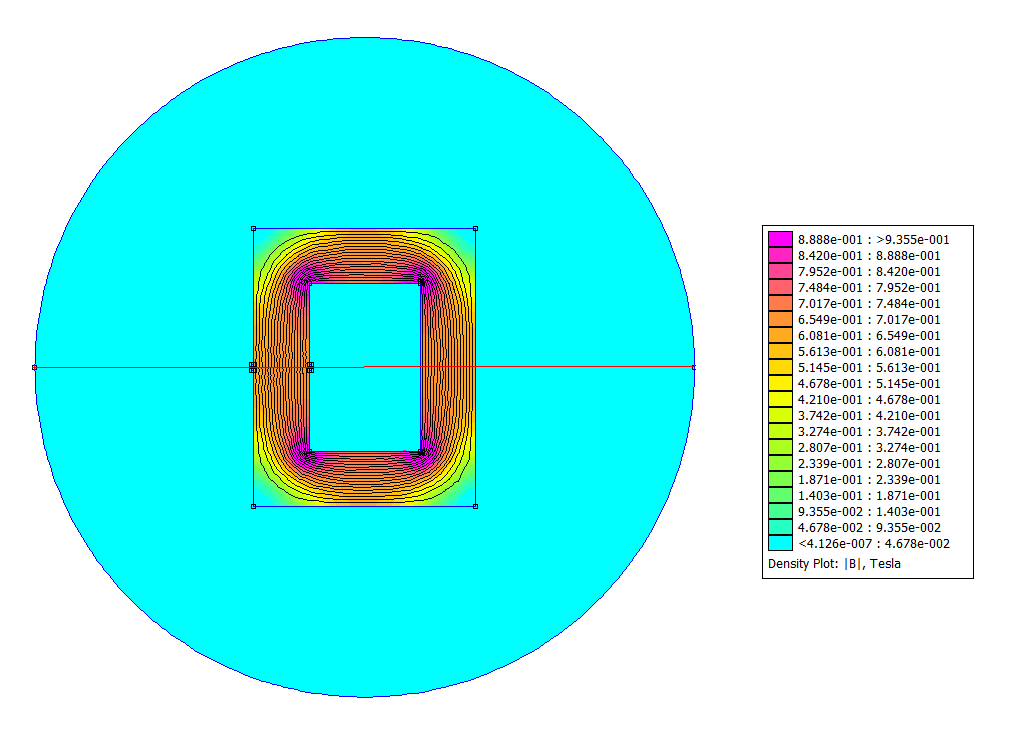
\includegraphics[scale=0.65]{img/assig1/femm2_4.png}
\caption[Densidade de fluxo (mapa de calor) e local de medição]{Densidade de fluxo (mapa de calor) e local de medição.}
\label{loc2_med}
\end{figure}

\begin{figure}[H]
\centering
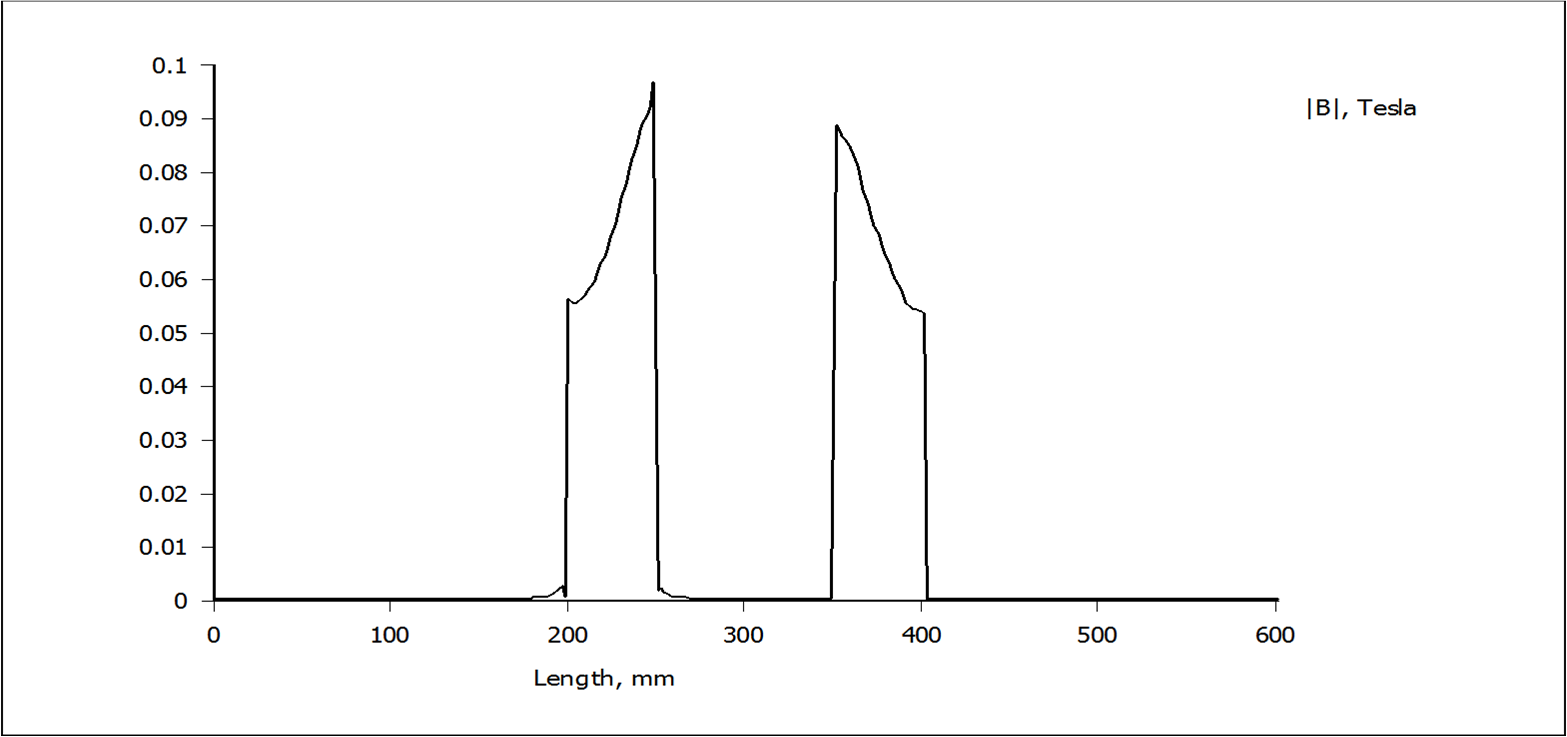
\includegraphics[scale=0.3]{img/assig1/linha_B.png}
\caption[Gráfico da densidade de fluxo magnético]{Gráfico da densidade de fluxo magnético.}
\label{graf2_dfm}
\end{figure}

\begin{figure}[H]
\centering
\includegraphics[scale=0.3]{img/assig1/linha_pot.png}
\caption[Gráfico do potencial]{Gráfico do potencial.}
\label{graf2_pot}
\end{figure}

\begin{figure}[H]
\centering
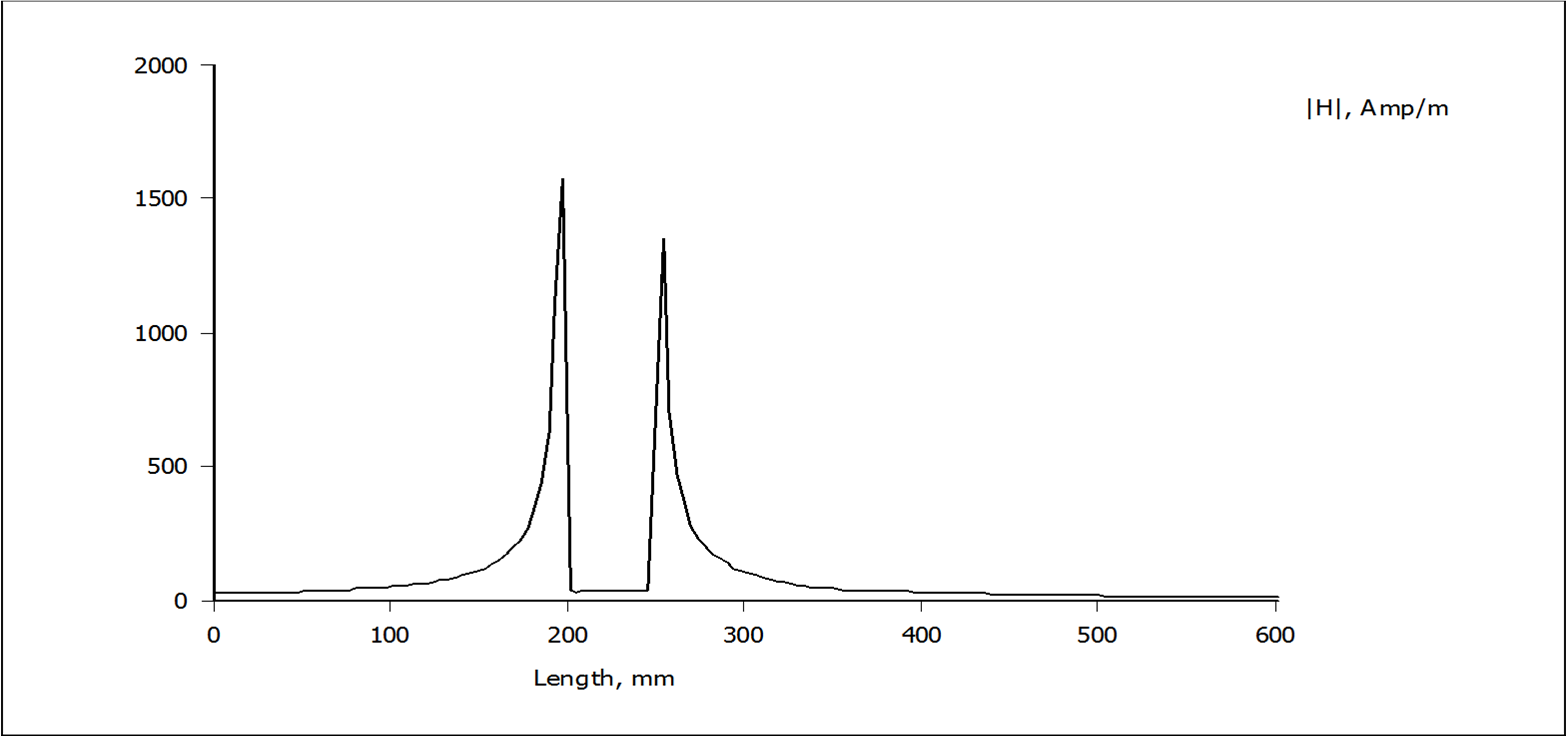
\includegraphics[scale=0.3]{img/assig1/linha_H.png}
\caption[Gráfico da intensidade de campo]{Gráfico da intensidade de campo.}
\label{graf2_ic}
\end{figure}
